\documentclass[a4paper,12pt]{report}

% Page layout
\usepackage[left=2.5cm,right=2.5cm,top=2.5cm,bottom=2.5cm]{geometry}

% Font and text
\usepackage[afrikaans,english]{babel}
\usepackage{microtype}
\usepackage{setspace}
\usepackage{lmodern}
\usepackage{siunitx}
\usepackage{ mathrsfs }
\newcommand{\myemph}[1]{{\sffamily\bfseries#1}}
\sloppy
\onehalfspacing

% Headings
\usepackage[raggedright,sf,bf]{titlesec}
\usepackage[margin=\the\parindent,small,bf,sf]{caption}
\titlelabel{\thetitle.\ }
\titleformat{\chapter}[display]{\huge\bfseries\sffamily}{\chaptertitlename\ \thechapter}{15pt}{\Huge \raggedright}
\titlespacing*{\chapter}{0pt}{0pt}{40pt}  % remove spacing before chapter headings
\makeatletter
\let\originall@chapter\l@chapter
\def\l@chapter#1#2{\originall@chapter{{\sffamily #1}}{#2}}
\makeatother

%% Alternative headings using small-caps (comment out the top section)
%\usepackage[raggedright,bf]{titlesec}
%\usepackage[margin=\the\parindent,small,bf]{caption}
%\titlelabel{\thetitle.\ }
%\titleformat{\chapter}[display]{\huge\scshape}{\chaptertitlename\ \thechapter}{15pt}{\Huge \raggedright}
%\titlespacing*{\chapter}{0pt}{0pt}{40pt}  % remove spacing before chapter headings

% Table of contents
\let \savenumberline \numberline
\def \numberline#1{\savenumberline{#1.}}

% Figures
\usepackage{graphicx}
\usepackage{pdfpages}
\usepackage{subcaption}
\setlength{\abovecaptionskip}{7.5pt}  % spacing above and below captions
\newcommand*{\WaterMark}[2][0.2\paperwidth]{\AddToShipoutPicture*{\AtTextCenter{\parbox[c]{0pt}{\makebox[0pt][c]{\includegraphics[width=#1]{#2}}}}}}

% Mathematics
\usepackage[cmex10]{amsmath}
\usepackage{amssymb}
\usepackage{cancel}
\DeclareMathOperator*{\argmax}{arg\,max}
\newcommand{\T}{^\top}
\newcommand{\tr}{\textrm{tr}}
\renewcommand{\vec}[1]{\boldsymbol{\mathbf{#1}}}
\newcommand{\defeq}{\triangleq}

% Tables
\usepackage{booktabs}
\usepackage{tabularx}
\usepackage{multirow}
\newcommand{\mytable}{
    \centering
    \small
    \renewcommand{\arraystretch}{1.2}
    }
\renewcommand{\tabularxcolumn}[1]{m{#1}}
\newcolumntype{C}{>{\centering\arraybackslash}X}
\newcolumntype{L}{>{\raggedright\arraybackslash}X}

% Header and footer
\usepackage{fancyhdr}
\pagestyle{fancy}
\fancyhf{}
\renewcommand{\sectionmark}[1]{\markright{\normalsize \thesection.\ #1}}
\fancyhead[C]{\nouppercase{\textit{\rightmark}}}
\fancyhead[RO]{\thepage}
 \fancyhead[LE]{\thepage}  % double-sided printing
\fancyfoot{}
\setlength\headheight{14.5pt}
\renewcommand{\headrulewidth}{0pt}
\fancypagestyle{plain}{\fancyhead{}
                       \renewcommand{\headrulewidth}{0pt}
                       \fancyfoot[C]{\thepage}}

% Pseudo-code
\usepackage{algorithm}  % should go before \usepackage{hyperref}

% Table of contents and hyperlinks
\usepackage{hyperref}
\hypersetup{colorlinks=true,linktoc=all,citecolor=black,linkcolor=black}
\usepackage[nottoc]{tocbibind}

% Pseudo-code
\usepackage{algpseudocode}  % should go after \usepackage{hyperref}
\renewcommand{\thealgorithm}{\arabic{chapter}.\arabic{algorithm}} 
\captionsetup[algorithm]{labelfont={bf,sf},font=small,labelsep=colon}

% Bibliography
\usepackage{cite}  % automatically reorder inline citations
\bibliographystyle{IEEEtran}

% Fix titlesec issue
\usepackage{etoolbox}
\makeatletter
\patchcmd{\ttlh@hang}{\parindent\z@}{\parindent\z@\leavevmode}{}{}
\patchcmd{\ttlh@hang}{\noindent}{}{}{}
\makeatother


\begin{document}

% Front matter
\graphicspath{{frontmatter/fig/}}
\pagenumbering{Alph}

\begin{titlepage}
	\begin{center}
		
		
\includegraphics[width=10cm]{USlogo-top}
		
		\vfill
		
		{\sffamily \bfseries \huge A Critical Analysis of Design Flaws in the Death Star \par}
%		{\scshape \huge A Critical Analysis of Design Flaws in the Death Star \par}
		
		\vfill
		
		{\large {\Large Luke Skywalker} \\ 99652154 \par}
		
		\vfill
		
		\vfill
		
		{Report submitted in partial fulfilment of the requirements of the module \\
			Project (E) 448 for the degree Baccalaureus in Engineering in the Department of
			Electrical and Electronic Engineering at Stellenbosch University. \par}
		
		\vfill
		
		{\large {Supervisor}: Dr O.\ W.\ Kenobi} %\\
		% Department of Electrical and Electronic Engineering \par}
		
		\vfill
		
		{\Large October 2099}
	\end{center}
\end{titlepage}

%\graphicspath{{frontmatter/fig/}}
\pagenumbering{Alph}

\begin{titlepage}
	\begin{center}
		
		%
\includegraphics[width=10cm]{USlogo-top}
		
		\WaterMark{UScrest-WM}
		
		~\vspace{4.5em}
		
		{\sffamily \bfseries \huge A Critical Analysis of Design Flaws in the Death Star \par}
%		{\scshape \huge A Critical Analysis of Design Flaws in the Death Star \par}		
		
		\vspace{7em}
		
		{\large {\Large  Luke Skywalker} \\ 99652154 \par}
		
		\vspace{8em}
		
		{\large Thesis presented in partial fulfilment of the requirements for the degree of \\ Master of Engineering (Electronic) in the Faculty of Engineering at Stellenbosch University. \par}
		
		\vfill
		
		{\large {Supervisor}: Dr O.\ W.\ Kenobi\\
		Department of Electrical and Electronic Engineering \par}
		
		%\vfill
		\vspace{10em}
		
		{\Large October 2099}
	\end{center}
\end{titlepage}

\pagenumbering{roman}
\chapter*{Acknowledgements}
% \addcontentsline{toc}{chapter}{Acknowledgements}
\makeatletter\@mkboth{}{Acknowledgements}\makeatother

<TODO: Do Really need this?>

I would like to thank my dog, Muffin. I also would like to thank the inventor of the incubator; without him/her, I would not be here. Finally, I would like to thank Dr Herman Kamper for this amazing report template.

%\chapter*{Declaration}
\newpage
\thispagestyle{plain}
\addcontentsline{toc}{chapter}{Declaration}
\makeatletter\@mkboth{}{Declaration}\makeatother

\centerline{
\includegraphics[width=8cm]{USlogo-top}}
\vspace*{-10pt}

\section*{\centering Plagiaatverklaring / \textit{Plagiarism Declaration}}

\vspace*{5pt}

\begin{enumerate}
    \item Plagiaat is die oorneem en gebruik van die idees, materiaal en ander intellektuele eiendom van ander persone asof dit jou eie werk is.\\
    \textit{Plagiarism is the use of ideas, material and other intellectual property of another's work
        and to present is as my own.}
    
    \item Ek erken dat die pleeg van plagiaat 'n strafbare oortreding is aangesien dit 'n vorm van diefstal is.\\
    \textit{I agree that plagiarism is a punishable offence because it constitutes theft.}
    
    \item Ek verstaan ook dat direkte vertalings plagiaat is. \\
    \textit{I also understand that direct translations are plagiarism.}
    
    \item Dienooreenkomstig is alle aanhalings en bydraes vanuit enige bron (ingesluit die internet) volledig verwys (erken). Ek erken dat die woordelikse aanhaal van teks sonder aanhalingstekens (selfs al word die bron volledig erken) plagiaat is. \\
    \textit{Accordingly all quotations and contributions from any source whatsoever (including the internet) have been cited fully. I understand that the reproduction of text without quotation marks (even when the source is cited) is plagiarism}
    
    \item Ek verklaar dat die werk in hierdie skryfstuk vervat, behalwe waar anders aangedui, my eie oorspronklike werk is en dat ek dit nie vantevore in die geheel of gedeeltelik ingehandig het vir bepunting in hierdie module/werkstuk of 'n ander module/werkstuk~nie. \\
    \textit{I declare that the work contained in this assignment, except where otherwise stated, is my original work and that I have not previously (in its entirety or in part) submitted it for grading in this module/assignment or another module/assignment.}
\end{enumerate}

\vfill

\noindent \begin{tabularx}{1.0\linewidth}{|L|L|}
    \hline
    \vspace{1cm} {Studentenommer / \textit{Student number}} & \vspace{1cm} {Handtekening / \textit{Signature}} \\
    \hline
    \vspace{1cm} {Voorletters en van / \textit{Initials and surname}} & \vspace{1cm} {Datum / \textit{Date}} \\
    \hline
\end{tabularx}

\vspace{15pt}

% The old declaration

%I, the undersigned, hereby declare that the work contained in this report is my own original work unless otherwise stated.
%
%% Afrikaans:
%% Hiermee verklaar ek, die ondergetekende, dat die werk in hierdie verslag vervat my eie oorspronklike werk is, tensy anders vermeld.
%
%\vspace{2.5cm}
%
%\begin{table}[h]
%\begin{tabular}{@{}p{2.5cm}p{5cm}}
%    Signature: & \dotfill \\
%    & \multicolumn{1}{c}{Obi-Wan Kenobi} \\
%    ~\vspace{1cm} \\
%    Date: & \dotfill \\
%\end{tabular}
%\end{table}
%
%\vfill
%
%\begin{center}
%    Copyright \textcopyright\ 2099 Stellenbosch University \\
%    All rights reserved
%\end{center}


\chapter*{Abstract}
\addcontentsline{toc}{chapter}{Abstract}
\makeatletter\@mkboth{}{Abstract}\makeatother

\subsubsection*{English}

The English abstract.

\selectlanguage{afrikaans}

\subsubsection*{Afrikaans}

Die Afrikaanse uittreksel.

\selectlanguage{english}
\tableofcontents
\listoffigures
\listoftables
\chapter*{Nomenclature\markboth{}{Nomenclature}}
\addcontentsline{toc}{chapter}{Nomenclature}

% \vspace*{-3mm}
\subsubsection*{Variables and functions}

\begingroup
\renewcommand{\arraystretch}{1.2}
\renewcommand{\tabularxcolumn}[1]{p{#1}}
\begin{tabularx}{\textwidth}{@{}p{2.5cm}L}
    $S_t$ & TODO \\
    $A_t^{(n)}$ & TODO \\
    $a_t^{(n)}$ & TODO \\
    $a_{i,j}$ & The probability of a transition from HMM state $s_i$ to state $s_j$. \\
    $b_i^{(n)}(j)$ & TODO. \\
    $p(x)$ & Probability density function with respect to variable $x$.\\
    $P(A)$ & Probability of event $A$ occurring.\\
    $\varepsilon$ & The Bayes error. \\
    $\varepsilon_u$ & The Bhattacharyya bound. \\
    $B$ & The Bhattacharyya distance. \\
    $s$ & An HMM state.  A subscript is used to refer to a particular state, e.g.\ $s_i$ refers to the $i^{\text{th}}$ state of an HMM. \\
    $\mathbf{S}$ & A set of HMM states. \\
    $\mathbf{F}$ & A set of frames. \\
    $\mathbf{o}_f$ & Observation (feature) vector associated with frame $f$. \\
    $\gamma_s(\mathbf{o}_f)$ & A posteriori probability of the observation vector $\mathbf{o}_f$ being generated by HMM state $s$. \\
    $\mu$ & Statistical mean vector. \\
    $\Sigma$ & Statistical covariance matrix. \\
    $L(\mathbf{S})$ & Log likelihood of the set of HMM states $\mathbf{S}$ generating the training set observation vectors assigned to the states in that set. \\
    $\mathcal{N}(\mathbf{x} | \mu, \Sigma)$ & Multivariate Gaussian PDF with mean $\mu$ and covariance matrix $\Sigma$.\\
    $N$ & Total number of frames or number of tokens, depending on the context. \\
    $D$ & Number of deletion errors. \\
    $I$ & Number of insertion errors. \\
    $S$ & Number of substitution errors. \\
\end{tabularx}
\endgroup


\newpage
\subsubsection*{Acronyms and abbreviations}

\begingroup
\renewcommand{\arraystretch}{1.2}
\begin{tabular}{@{}p{2.5cm} l}
    DNBC    & Dynamic Naive Bayes Classifier \\
    AE      & Afrikaans English \\
    AID     & accent identification \\
    ASR     & automatic speech recognition \\
    AST     & African Speech Technology \\
    CE      & Cape Flats English \\
    DCD     & dialect-context-dependent \\
    DNN		& deep neural network \\
    G2P     & grapheme-to-phoneme \\
    GMM     & Gaussian mixture model \\
    HMM     & hidden Markov model \\
    HTK     & Hidden Markov Model Toolkit \\
    IE      & Indian South African English \\
    IPA     & International Phonetic Alphabet \\
    LM      & language model \\
    LMS     & language model scaling factor \\
    MFCC    & Mel-frequency cepstral coefficient \\
    MLLR    & maximum likelihood linear regression \\
    OOV     & out-of-vocabulary \\
    PD      & pronunciation dictionary \\
    PDF     & probability density function \\
    SAE     & South African English \\
    SAMPA   & Speech Assessment Methods Phonetic Alphabet \\
\end{tabular}
\endgroup

\newpage
\pagenumbering{arabic}

% Contents
\graphicspath{{introduction/fig/}}

\chapter{Introduction}
\label{chap:introduction}

The last few years have seen great advances in speech recognition. Much of this progress is due to the resurgence of neural networks; most speech systems now rely on deep neural networks (DNNs) with millions of parameters~\cite{dahl+etal_taslp12,hinton+etal_spm2012}.
However, as the complexity of these models has grown, so has their reliance on labelled training data. Currently, system development requires large corpora of transcribed speech audio data, texts for language modelling, and pronunciation dictionaries.
Despite speech applications becoming available in more languages, it is hard to imagine that resource collection at the required scale would be possible for all 7000 languages spoken in the world today.

I really like apples.

\section{Section heading}

This is some section with two table in it: Table~\ref{tbl:exemplars} and Table~\ref{tbl:abx_speaker}.

\begin{table}[!h]
    \mytable
    \caption{Performance of the unconstrained segmental Bayesian model on TIDigits1 over iterations in which the reference set is refined.}
    \begin{tabularx}{\linewidth}{@{}lCCCCC@{}}
        \toprule
        Metric     & 1 & 2 & 3 & 4 & 5 \\
        \midrule
        WER (\%)                        & $35.4$ & $23.5$ & $21.5$ & $21.2$ & $22.9$ \\
        Average cluster purity (\%)       & $86.5$ & $89.7$ & $89.2$ & $88.5$ & $86.6$ \\
        Word boundary $F$-score (\%)         & $70.6$ & $72.2$ & $71.8$ & $70.9$ & $69.4$ \\
        Clusters covering 90\% of data   & 20             & 13 & 13 & 13 & 13 \\
        \bottomrule
    \end{tabularx}
    \label{tbl:exemplars}
\end{table}


\begin{table}[!h]
    \renewcommand{\arraystretch}{1.1}
    \centering
    \caption{A table with an example of using multiple columns.}
    \begin{tabularx}{0.65\linewidth}{@{}lCCr@{}}
        \toprule
        & \multicolumn{2}{c}{Accuracy (\%)} \\
        \cmidrule(lr){2-3}
        Model    & Intermediate & Output & Bitrate\\
        \midrule
        Baseline & 27.5         & 26.4   & 116 \\
        VQ-VAE   & 26.0         & 22.1   & 190 \\
        CatVAE   & 28.7         & 24.3   & 215 \\
        \bottomrule
    \end{tabularx}
    \label{tbl:abx_speaker}
\end{table}

\newpage

This is a new page, showing what the page headings looks like, and showing how to refer to a figure like Figure~\ref{fig:cae_siamese}.

\begin{figure}[!t]
    \centering
%     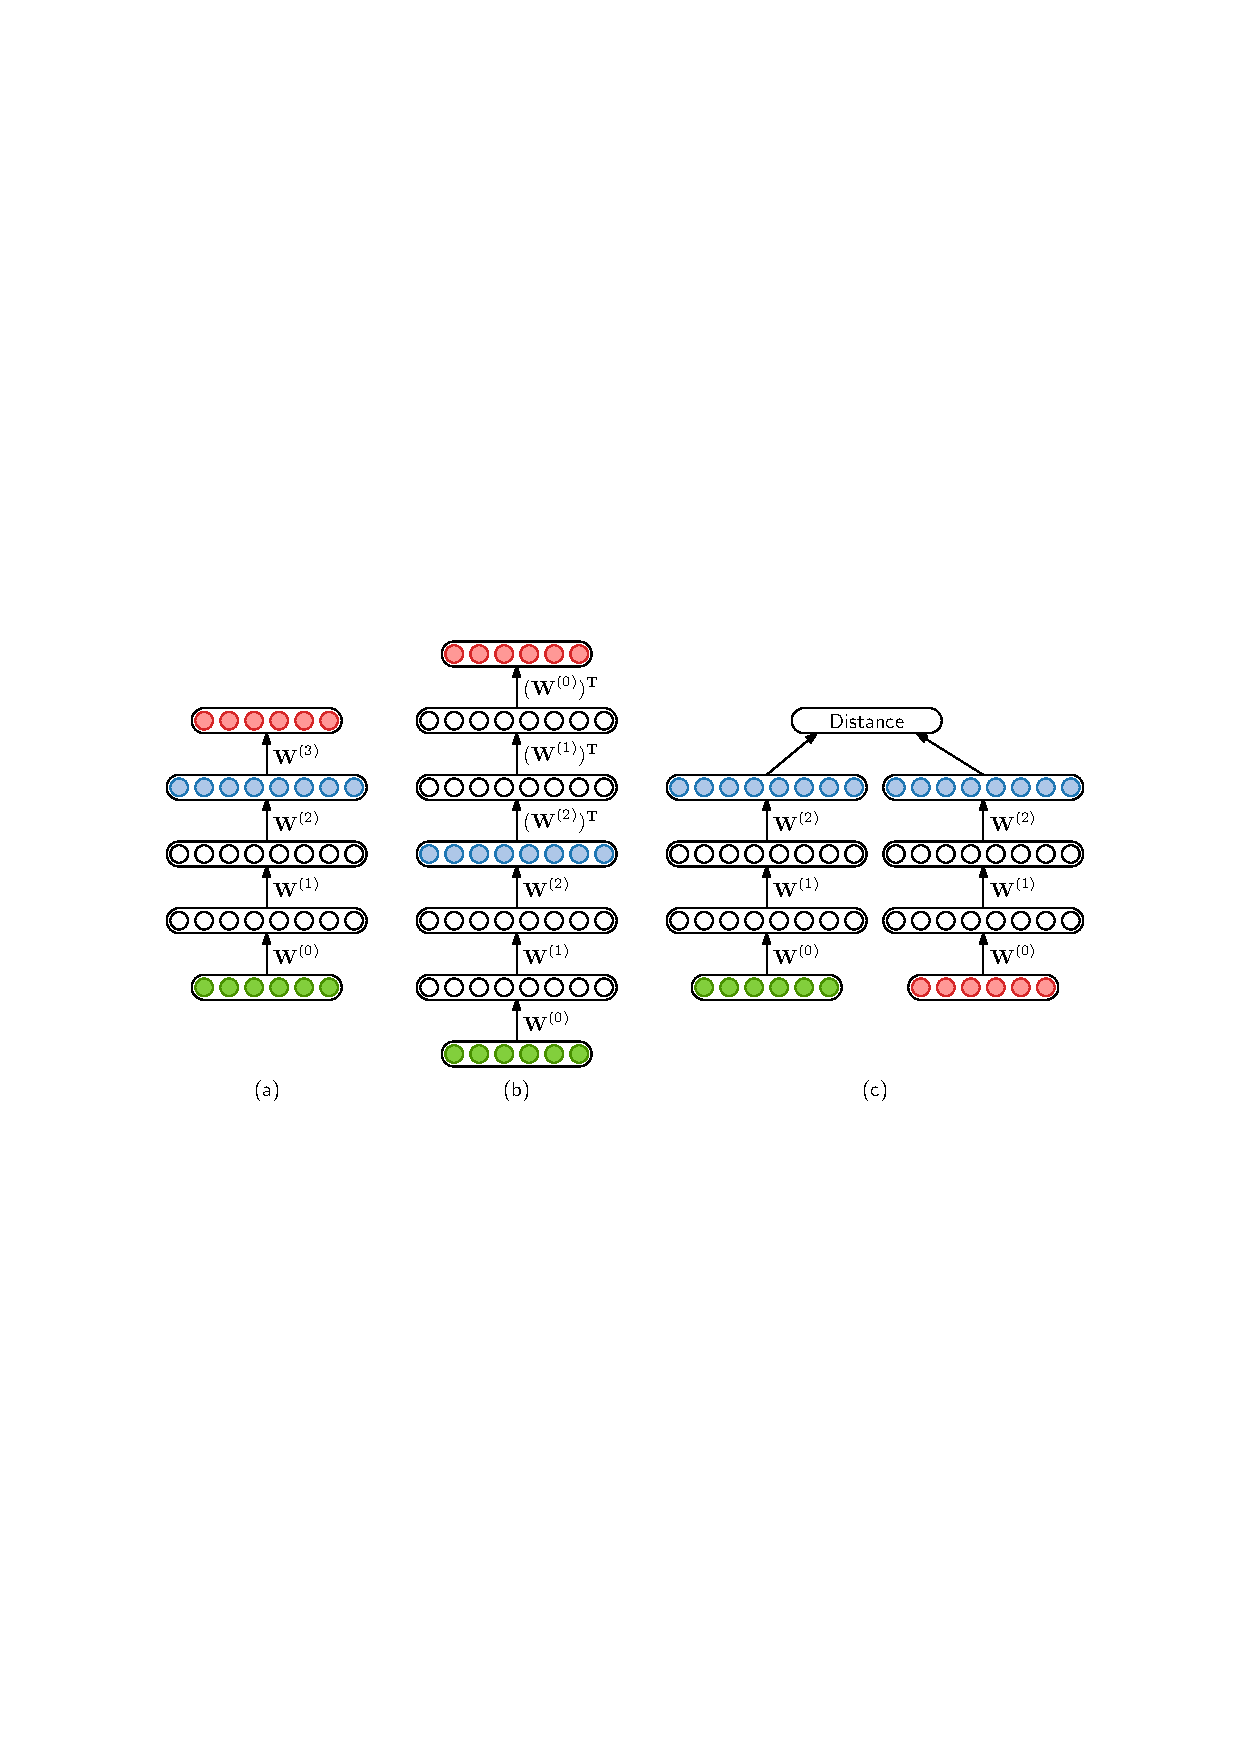
\includegraphics[width=\linewidth]{cae_siamese}
    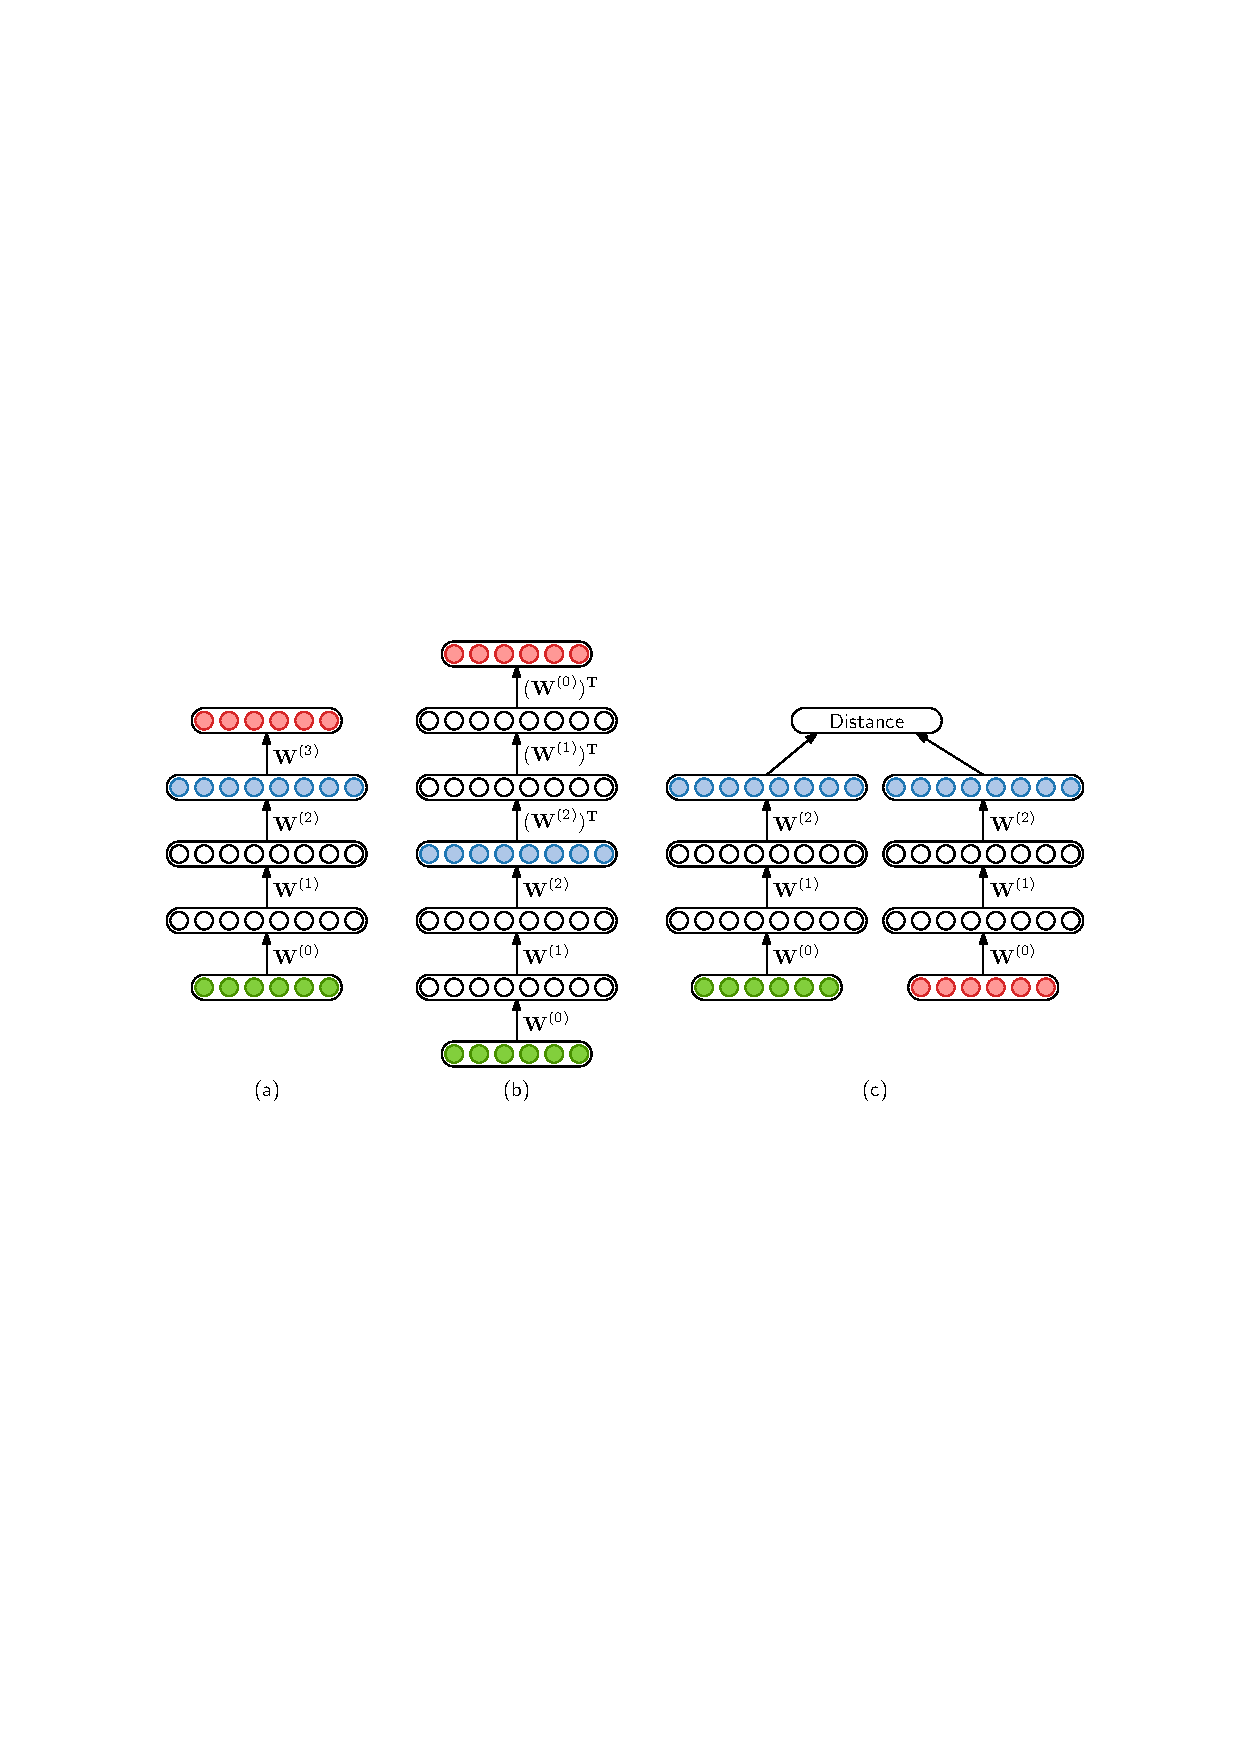
\includegraphics[width=0.918\linewidth]{cae_siamese}
    \caption[I am the short caption that appears in the list of figures, without references.]{
    (a) The cAE as used in this chapter. The encoding layer (blue) is chosen based on performance on a development set.
    (b) The cAE with symmetrical tied weights. The encoding from the middle layer (blue) is always used.
    (c) The siamese DNN. The cosine distance between aligned frames (green and red) is either minimized or maximized depending on whether the frames belong to the same (discovered) word or not.
    A cAE can be seen as a type of DNN~\cite{dahl+etal_taslp12}.
    }
    \label{fig:cae_siamese}
\end{figure}


The following is an example of an equation:
\begin{equation}
P(\vec{z} | \vec{\alpha}) = \int_{\vec{\pi}} P(\vec{z} | \vec{\pi}) \, p(\vec{\pi} | \vec{\alpha}) \, \textrm{d} \vec{\pi}
= \int_{\vec{\pi}} \prod_{k = 1}^K \pi_k^{N_k} \frac{1}{B(\vec{\alpha})} \prod_{k = 1}^K \pi_k^{\alpha_k - 1} \, \textrm{d} \vec{\pi}
\label{eq:example_equation}
\end{equation}
which you can subsequently refer to as~\eqref{eq:example_equation} or Equation~\ref{eq:example_equation}.
But make sure to consistently use the one or the other (and not mix the two ways of referring to equations).

\graphicspath{{body/fig/}}

\chapter{Body}
\label{chap:body}

\section{Model Definition}

\begin{figure}[!h]
    \centering
    \includegraphics[width=\linewidth]{model-drawing.png}
    \caption[I am the short caption that appears in the list of figures, without references.]{ I am a caption below the figure of course}
    \label{fig:model-drawing}
\end{figure}

RVs:
\begin{itemize}
    \item Hidden Drought State RVs $\equiv S_t = \{1,2,\dots,m\}$    
    \item Attribute RVs $\equiv A^{(n)}_t = \{1,2,\dots,C_n\}$
\end{itemize}

Some further notation:
\begin{itemize}
    \item $\vec{S}_{1:T}  = \{S_1,S_2,\dots,S_T\}$    
    \item $A_{1:T} = \{\vec{A}_1,\vec{A}_2,\dots,\vec{A}_T\}$
    \begin{itemize}
        \item Where $\vec{A}_t = \{ A^{(1)}_t, A^{(2)}_t, \dots, A^{(N)}_t\}$
    \end{itemize}
\end{itemize}


\subsection{Joint Distribution}

\[
\begin{align}
    &p(S_1, S_2, \dots, S_T, A^{(1)}_1, A^{(2)}_1, \dots, A^{(N)}_1, A^{(1)}_2, \dots, A^{(N)}_T) \\ 
    &= p(S_1, S_2, \dots, S_T, \vec{A}_1, \vec{A}_2, \dots, \vec{A}_T) \\
    &= p(\vec{S}_{1:T}, A_{1:T}) \\
    &= p(S_1) \cdot \prod\limits_{t=1}^{T-1} p(S_{t+1} \mid S_t) \cdot \prod\limits_{n=1}^{N} \prod\limits_{t=1}^T p(A^{(n)}_t \mid S_t)
\end{align}
\]

\section{Factors}

Priors
\[
\begin{array}{c | c}
S_1 & p(S_1) \\ 
\hline
1 & \pi_1 \\ 
2 & \pi_2 \\ 
\vdots & \vdots \\
m & \pi_m \\ 
\end{array} 
\]

Transition
\[
\begin{array}{ccc}
\begin{array}{c c | c}
S_t & S_{t+1} & p(S_{t+1} \mid S_t) \\ 
\hline
1 & 1  & a_{1,1} \\ 
1 & 2  & a_{1,2} \\ 
\vdots & \vdots  & \vdots \\
1 & m  & a_{1,m} \\ 
2 & 1  & a_{2,1} \\ 
2 & 2  & a_{2,2} \\ 
\vdots & \vdots  & \vdots \\
m & m  & a_{m,m} \\ 
\end{array} 
&
\equiv
&
P^1 = 
\begin{bmatrix}
a_{1,1} & a_{1,2} & \dots & a_{1,m} \\
a_{2,1} & a_{2,2} & \dots & a_{2,m} \\
\vdots & \vdots & \ddots & \vdots \\
a_{m,1} & a_{m,2} & \dots & a_{m,m} \\
\end{bmatrix}
\end{array} 
\]


Emission
\[
\begin{array}{c c | c}
A^{(n)}_t & S_t & p(A^{(n)}_t \mid S_t) \\ 
\hline
1 & 1  & b_1^{(n)}(1) \\ 
1 & 2  & b_2^{(n)}(1) \\ 
\vdots & \vdots  & \vdots \\
1 & m  & b_m^{(n)}(1) \\ 
2 & 1  & b_1^{(n)}(2) \\ 
2 & 2  & b_2^{(n)}(2) \\ 
\vdots & \vdots  & \vdots \\
C_n & m  & b_m^{(n)}(C_n) \\ 
\end{array} 
\]

\newpage

\section{Update Equations}
Priors:
\begin{equation}
\pi_i^{\text{new}} = q(S_1=i)
\label{eq:prior_update}
\end{equation}

Transition Probabilities:
\begin{equation}
a_{ij}^{\text{new}} = \frac{\sum\limits_{t=1}^{T - 1} q(S_t=i,S_{t+1}=j)}{\sum\limits_{t=1}^{T-1} q(S_t=i)}
\label{eq:transition_update}
\end{equation}


Emission Probabilities:
\begin{equation}
b_i^{(n)}(j)^{\text{new}} = \frac{\sum\limits_{t=1}^T q(S_t = i) \cdot I(A_t^{(n)} = j)}{\sum\limits_{t=1}^T q(S_t = i)}
\label{eq:emission_update}
\end{equation}

We can now reference these equations by their label: Equation~\ref{eq:prior_update}, Equation~\ref{eq:transition_update} or Equation~\ref{eq:emission_update}. This is wicked, lemme tell you

\newpage

\section{FIGURES TIME}

things before figure

We can also reference this guy with a cheeky Figure~\ref{fig:model-drawing}


\section{Determining $m$}

Okay some questions:
\begin{enumerate}
    \item I have one sequence of $T$ observations with $N$ variables being observed at each $t$ step. Would my $k$ then be $T \times N$ or would it just be $T$?
    \item Define, algebraically, exactly what my $L$ should be that I need to calculate
\end{enumerate}

Okay progress update:
I have built the model. I have used synthetic data for model development. We have:


Note: Our attribute RVs are discrete. 

Model works with a set $m$ but the paper estimates this value using maximized log-likelihood, AIC and BIC
How do i do this? Is it just creating the model for various values of $m$ and choosing the one that returns the lowest AIC, BIC and largest log-likelihood?




 Consequently, in analyzing the drought indices, the number of latent states m was the first quantity we wanted to extract. We considered a simple procedure based on information criteria, which is a usual tool for model selection. The model with the optimal number of latent states was expected to best explain the data with a minimum number of free parameters. We used the  given as follows:
\[
    AIC = -2 \hspace{0.1cm} \text{log} L + 2p
\]

\[
    BIC = -2 \hspace{0.1cm}\text{log}L + p \text{log} k
\]

Where $L \equiv$ the maximized value of the likelihood function for the estimated model

$p \equiv$ the number of free parameters, 

$k \equiv$ the number of data points. 




\graphicspath{{conclusion/fig/}}

\chapter{Summary and Conclusion}
\label{chap:conclusion}

\paragraph{TODO: NOT FINISHED}
While it doesn't appear to be a complete success, it provides valuable insights into the behavior and limitations of the Dynamic Naive Bayes Classifier (DNBC) for this task.
 The model's rapid switching does not reflect this physical reality, suggesting it may be over-reacting to short-term noise in the input data rather than capturing the underlying climatological state.

## Conclusion on Model Performance

In summary, the DNBC, as implemented, demonstrates a partial ability to detect drought conditions. It successfully identifies recent, severe droughts but struggles with consistency and stability across the entire historical record.

Its primary limitations are an **unrealistic temporal volatility** and a **high rate of false alarms**. These results suggest that while the model is capturing some relevant signals, it is either overly sensitive to noise in the input indicators or the model structure itself (e.g., the assumptions of the Naive Bayes classifier or the learned transition probabilities) is not robust enough to represent the persistent nature of drought. Further refinement, such as temporal smoothing of the output or incorporating model parameters that enforce state persistence, would be necessary to improve its practical utility as a composite indicator.


\textbf{Summary:}  
The DNBC model, with $m = 6$ latent states, successfully encapsulates the cyclical nature of South African drought dynamics. While the temporal output remains somewhat oscillatory due to noisy inputs, the probabilistic framework provides a balanced and interpretable representation of drought evolution. Quantitatively, the model outperforms the individual indices across key performance metrics, confirming that combining multiple drought sources via latent-state modelling yields a modest but meaningful improvement in predictive robustness.


% Bibliography
\bibliography{mybib}

% End matter
\appendix
\chapter{Project Planning Schedule}
\makeatletter\@mkboth{}{Appendix}\makeatother
\label{appen:derivations_bigramseg}

This is an appendix.

\chapter{Outcomes Compliance}
\makeatletter\@mkboth{}{Appendix}\makeatother
\label{appen:derivations_bigramseg}

This is another appendix.

\end{document}

